% coding:utf-8

%FOSASTOC, a LaTeX-Code for a electrical summary of stochastic
%Copyright (C) 2013, Daniel Winz, Ervin Mazlagic

%This program is free software; you can redistribute it and/or
%modify it under the terms of the GNU General Public License
%as published by the Free Software Foundation; either version 2
%of the License, or (at your option) any later version.

%This program is distributed in the hope that it will be useful,
%but WITHOUT ANY WARRANTY; without even the implied warranty of
%MERCHANTABILITY or FITNESS FOR A PARTICULAR PURPOSE.  See the
%GNU General Public License for more details.
%----------------------------------------

\chapter{Kombinatorik}
\newpage

\section{Logik \& Mengenlehre}
Die Logik ist ein Teilgebiet der Mathematik und bedgründete das relativ
junge Teilgebiet der \gls{Mengenlehre} (engl. \emph{set theory}). 
Dass diese beiden Teilgebiete sich sehr ähnlich sind, zeigt sich 
unter anderem in ihren ähnlichen Notationen.

Die Mengenlehre zeichnet sich insbesondere dadurch aus, 
dass es eine starke \gls{Abstraktion} zulässt.
Diese Eigenschaft ermöglicht es die Mengenlehre für viele Probleme
heranzuziehen. Die Stochastik ist nur eines von diesen.

\begin{table}[h!]
	\centering
	\begin{tabular}{l c |l c}
		Aussagelogik 
			& 
			& Mengenlehre 
			& \\
		\hline
		& & & \\
		Konjunktion
			& $A \land B$
			& Schnittmenge
			& $A \cap B$ \\
		& & & \\
		Disjunktion
			& $A \lor B$
			& Vereinigung
			& $A \cup B$ \\
		& & & \\
		Logische Äquivalenz
			& $A \Leftrightarrow B$
			& Differenzmenge
			& $A \setminus B$ \\
		& & & \\
		Implikation
			& $A \Rightarrow B$  
			& Symmetrische Differenz
			& $A \triangle B$ \\
		& & & \\
		Kontravalenz
			& $A \veebar B$ 
			& Disjunkte Vereinigung
			& $A \dot\cup B$ \\
		& & & \\
		Negation
			& $\bar{A}$
			& Komplement 
			& $A^{\mathrm C}$ \\
		& & & \\
	\end{tabular}
	\caption{Junktoren der Logik und Operationen der 
		Mengenlehre}
\end{table}

\subsection{Begriffe der Mengenlehre}
\paragraph{Grundmenge und Grundraum}
In der Mengenlehre spricht man von der Grundmenge als die Menge aller
möglicher Elemente die in einer Menge erfasst werden können (von Neumann
Universum etc). Im Teilgebiet der Stochastik betrachtet man die
Elemente die in Mengen erfasst werden können als Eereignisse die eintreten
können. Die Gesamtheit all dieser möglichen Ereignisse nennt man 
\gls{Ereignisraum} oder Grundmenge, welche stets mit $\Omega$ 
notiert wird. 
Bei der Betrachtung eines Spiels mit einem Spielwürfel mit sechs Seiten 
wäre der Grundraum $\Omega=\{1,2,3,4,5,6\}$ und bei einem zweifachen
Münzwurf $\Omega=\{KK, KZ, ZK, ZZ\}$ usw.
\[  
	\Omega := \{x| P(x) \neq 0\}
\]

\paragraph{Teilmenge} 
Eine Menge $A$ heisst \gls{Teilmenge} von $B$, wenn jedes Element aus 
$A$ ein Element von $B$ ist. Somit kann eine solche Teilmenge $A$
auch die ganze Menge $B$ sein, d.h. es kann $A=B$ gelten.
\[ 
	A \subseteq B
\]
\paragraph{Echte Teilmenge}
Eine \gls{echte Teilmenge} $A$ der Menge $B$ heisst echte Teilmenge, wenn
alle Elemente von $A$ in $B$ enthalten sind, aber die Menge $B$ noch
Elemente hat, die nicht in $A$ enthalten sind. In diesem Fall ist $B$ 
auch eine \emph{echte} Obermenge von $A$ und es gilt $A \neq B$.
\[
	A \subset B
\]

\paragraph{Leere Menge} Eine \gls{leere Menge} ist eine Menge welche 
keinerlei Elemente enthält. Sie wird entweder als $\{ \}$ oder 
$\emptyset$ notiert.
\[  
	A = \{\} = \emptyset
\]

\paragraph{Schnittmenge} Eine Menge von Elementen die allesamt sowohl in
der Menge $A$ als auch in der Menge $B$ vorkommen, wird \gls{Schnittmenge} 
dieser Mengen genannt.
\[ 
	A \cap B
\]

\paragraph{Vereinigungsmenge} Die Menge aller Elemente die entweder in
der Menge $A$, in der Menge $B$ oder in beiden Mengen $A,B$ vorkommen,
wird als \gls{Vereinigungsmenge} bezeichnet.
\[  
	A \cup B
\]

\paragraph{Gleiche Menge} Wenn zwei Mengen die gleichen Elemente
enthalten und keine weiteren, so sind diese die \gls{gleiche Menge}.
\[  
	A = B 
	\quad \Leftrightarrow \quad 
	\forall x (x \in A \leftrightarrow x \in B)
\]

\paragraph{Differenzmenge}
Eine Menge die alle Elemente einer Menge enthält ohne jene die auch
in einer weiteren Menge vorkommen, wird als \gls{Differenzmenge} 
bezeichnet.
\[
	A \setminus B 
\]

\paragraph{Potenzmenge}
Für eine Menge $\Omega$ gibt es die sogenannte \gls{Potenzmenge} 
$\mathcal{P}(\Omega)$, welche alle Teilmengen $\omega$ von $\Omega$ 
beschreibt.
Eine Potenzmenge ist also per Definition eine Menge, welche nur
aus Mengen besteht. 

Die Potenzmenge kennt eine Reihe von gebräuchlichen
Notationen wobei $\mathcal{P}(\Omega)$ die gängigste ist. Weitere 
Notationen sind z.B. $\mathfrak{P}(\Omega)$ oder auch
$\prod(\Omega)$
\[ 
	\mathcal{P}(\Omega) 
		\quad = \quad \{\omega \mid \omega \subseteq \Omega \}
\]

\begin{figure}[h!]
	\centering
	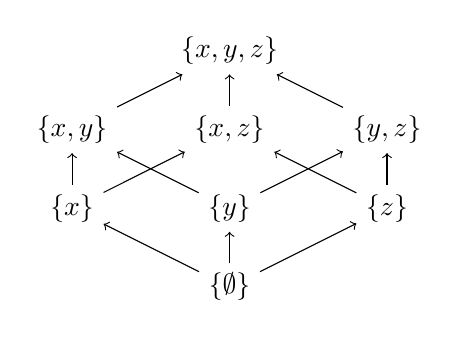
\begin{tikzpicture}
		\node (pot) 	at ( 0.0, 0.0) 	{$\{\emptyset\}$};
		\node (x) 	at (-2.0, 1.0) 	{$\{x\}$};
		\node (y)	at ( 0.0, 1.0) 	{$\{y\}$};
		\node (z)	at ( 2.0, 1.0) 	{$\{z\}$};
		\node (xy) 	at (-2.0, 2.0) 	{$\{x,y\}$};
		\node (xz)	at ( 0.0, 2.0) 	{$\{x,z\}$};
		\node (yz)	at ( 2.0, 2.0) 	{$\{y,z\}$};
		\node (xyz)	at ( 0.0, 3.0)	{$\{x,y,z\}$};
		\draw[->] (pot) -- (x);
		\draw[->] (pot) -- (y);
		\draw[->] (pot) -- (z);
		\draw[->] (x) -- (xy);
		\draw[->] (x) -- (xz);
		\draw[->] (y) -- (xy);
		\draw[->] (y) -- (yz);
		\draw[->] (z) -- (xz);
		\draw[->] (z) -- (yz);
		\draw[->] (xy) -- (xyz);
		\draw[->] (xz) -- (xyz);
		\draw[->] (yz) -- (xyz);
	\end{tikzpicture}
	\caption{Potenzmenge von $\{x,y,z\}$ als Hasse-Diagramm}
\end{figure}

\paragraph{Komplement}
Eine Menge welche alle Elemente aus einer Potenzmenge 
$\mathcal{P}(\Omega)$
enthält ohne Elemente einer Menge $A\in\Omega$ heisst \gls{Komplement} der 
Menge $A$ und wird als $A^\mathrm C$ notiert\footnote{Das Komplement in 
der Mengenlehre sollte stets als $A^{\mathrm C}$ notiert werden obwohl
oft diverse andere Schreibweisen anzutreffen sind wie z.B. $\bar{A}$.}. 
Somit kann ein Komplement 
als Differenzmenge einer Potenzmenge und einer Menge beschrieben werden.
\[  
	A^{\mathrm C} 
		\quad = \quad \Omega \setminus A 
		\quad := \quad \{\omega\in\Omega \mid \omega\notin A\} 
			\in\mathcal{P}(\Omega)
\]

\newpage
\begin{figure}[h!]
	\centering
	\begin{subfigure}[b]{0.45\textwidth}
		\centering
		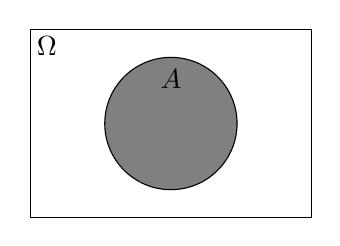
\begin{tikzpicture}[scale=0.7]
			\fill[white] (-2.55,-1.7) rectangle (2.55,1.7);
			\draw (-2.55,-1.7) rectangle (2.55,1.7);
			\fill[gray] (0,0) circle (1.2cm);
			\draw (0,0) circle (1.2cm);
			\draw (0,0.8) node {$A$};
			\node at (-2.25, 1.4) {$\Omega$};
		\end{tikzpicture}
		\caption{$A$}
	\end{subfigure}
	\begin{subfigure}[b]{0.45\textwidth}
		\centering
		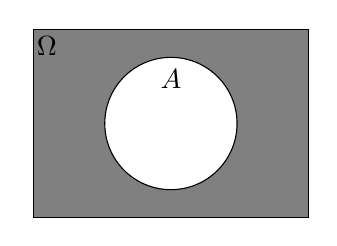
\begin{tikzpicture}[scale=0.7]
			\fill[gray] (-2.5,-1.7) rectangle (2.5,1.7);
			\draw (-2.5,-1.7) rectangle (2.5,1.7);
			\fill[white] (0,0) circle (1.2cm);
			\draw (0,0) circle (1.2cm);
			\draw (0,0.8) node {$A$};
			\node at (-2.25, 1.4) {$\Omega$};
		\end{tikzpicture}
		\caption{$A^{\mathrm C}$}
	\end{subfigure}

	\rule[1mm]{0mm}{5mm}

	\begin{subfigure}[b]{0.45\textwidth}
		\centering
		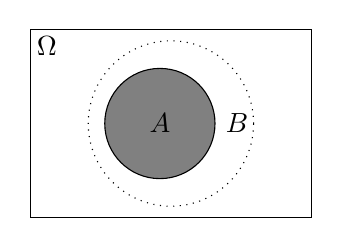
\begin{tikzpicture}[scale=0.7]
			\fill[white] (-2.55,-1.7) rectangle (2.55,1.7);
			\draw (-2.55,-1.7) rectangle (2.55,1.7);
			\draw[dotted] (0,0) circle (1.5cm);
			\fill[gray] (-0.2,0) circle (1cm);
			\draw (-0.2,0) circle (1cm);
			\draw (-0.2,0) node {$A$};
			\draw (1.2,0) node {$B$};
			\node at (-2.25, 1.4) {$\Omega$};
		\end{tikzpicture}
		\caption{$A \subseteq B$}
	\end{subfigure}
	\begin{subfigure}[b]{0.45\textwidth}
		\centering
		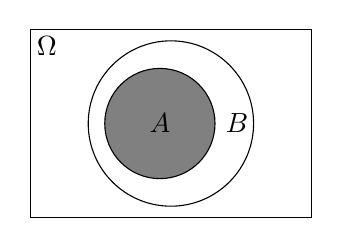
\begin{tikzpicture}[scale=0.7]
			\fill[white] (-2.55,-1.7) rectangle (2.55,1.7);
			\draw (-2.55,-1.7) rectangle (2.55,1.7);
			\draw (0,0) circle (1.5cm);
			\fill[gray] (-0.2,0) circle (1cm);
			\draw (-0.2,0) circle (1cm);
			\draw (-0.2,0) node {$A$};
			\draw (1.2,0) node {$B$};
			\node at (-2.25, 1.4) {$\Omega$};
		\end{tikzpicture}
		\caption{$A \subset B$}
	\end{subfigure}

	\rule[1mm]{0mm}{5mm}

	\begin{subfigure}[b]{0.45\textwidth}
		\centering
		\begin{venndiagram2sets}[tikzoptions={scale=0.7}]
    			\fillACapB;
			\node at (0.3, 3.1) {$\Omega$};
		\end{venndiagram2sets}
		\caption{$A \cap B$}
	\end{subfigure}
	\begin{subfigure}[b]{0.45\textwidth}
		\centering
		\begin{venndiagram2sets}[tikzoptions={scale=0.7}]
			\fillNotAorNotB;
			\node at (0.3, 3.1) {$\Omega$};
		\end{venndiagram2sets}
		\caption{${(A\cap B)}^{\mathrm C}$}
	\end{subfigure}

	\rule[1mm]{0mm}{5mm}

	\begin{subfigure}[b]{0.45\textwidth}
		\centering
		\begin{venndiagram2sets}[tikzoptions={scale=0.7}]
			\fillA \fillB;
			\node at (0.3, 3.1) {$\Omega$};
		\end{venndiagram2sets}
		\caption{$A \cup B$}
	\end{subfigure}	
	\begin{subfigure}[b]{0.45\textwidth}
		\centering
		\begin{venndiagram2sets}[tikzoptions={scale=0.7}]
			\fillNotAorB;
			\node at (0.3, 3.1) {$\Omega$};
		\end{venndiagram2sets}
		\caption{${(A \cup B)}^{\mathrm C}$}
	\end{subfigure}
	\caption{Die wichtigsten Operationen der Mengenlehre graphisch
	erläutert mittels Venn-Diagrammen für $A,B \subset \Omega$.}
\end{figure}

\section{Kombinatorik}
Im Teilgebiet der Stochastik gibt es einige Regeln die es in der 
Kombinatorik zu beachten gilt. Insbesondere sind dies die 
\gls{Axiome von Kolmogorov}.

\subsection{Axiome von Kolmogorov}
Der russische Mathematiker Andrei Nikolajevitsch \gls{Kolmogorov} 
definierte drei Axiome für die Wahrscheinlichkeitstheorie.
\begin{enumerate}
	\item \textbf{\gls{Nichtnegativitaet}} \\
		Jedes Ereignis $A$ aus der Ergebnismenge $\Omega$ hat eine 
		reelle Eintrittswahrscheinlichkeit $P(A)$ von 
		$P(A) \geq 0$. Das bedeutet insbesondere, dass es 
		keine negativen Wahrscheinlichkeiten gibt.
		\[ P(A) \geq 0 \quad \text{für } A \in \Omega \] 
	\item \textbf{\gls{Normiertheit}} \\
		Das sichere Ereignis der Ergebnismenge $\Omega$ hat eine
		Wahrscheinlichkeit von $P(\Omega)=1$. Dies sagt aus, dass
		sich immer etwas ereignen wird und dass das unmögliche
		Ereignis, die Wahrscheinlichkeit $P(\emptyset)=0$ hat.
		\[ P(\Omega) = 1 \]
	\item \textbf{\gls{Additivitaet}} \\
		Die Wahrscheinlichkeit einer Vereinigung disjunkter 
		Ereignisse ist gleich der Summe der einzelnen 
		Wahrscheinlichkeiten. Dies kann als 
		$P(A_1 \dot\cup A_2  \dots ) = \sum P(A_i)$ 
		formuliert werden und wird als $\sigma$-Additivität
		bezeichnet.
		\[ P(A+B) = P(A)+P(B) \quad \text{falls } A \cap B = 0 \]
\end{enumerate}

\subsection{Stochastisch unabhängige Ereignisse}
Hat man zwei Ereignisse $A,B$ welche die nachfolgende Definition erfüllen
so nennt man diese \gls{stochastisch unabhaengig}.
\[ \left. 
	\begin{array}{l c l}
		P(A|B)
			& =
			& P(A) \\
		& & \\
		P(B|A)
			& =
			& P(B) \\
	\end{array} \right\}
	\Rightarrow P(A) \cdot P(B)
\]
Die allgemeingültige mathematische Definition der stochastischen 
Unabhängigkeit ist
etwas umständlich, kann aber einfach erläutert werden und lässt zu,
die Unabhängigkeit von beliebig vielen Ereignissen zu prüfen.

Im Falle von drei Ereignissen $A,B,C$ muss zur stochastischen
Unabhängigkeit folgendes gelten
\[ \begin{array}{r c l}
	P(A \cap B)
		& = 
		& P(A) \cdot P(B) \\
	& & \\
	P(A \cap C)
		& =
		& P(A) \cdot P(C) \\
	& & \\
	P(B \cap C)
		& =
		& P(B) \cdot P(C) \\
	& & \\
	P(A \cap B \cap C)
		& =
		& P(A) \cdot P(B) \cdot P(C)
\end{array} \]
Hier lässt sich nun etwas deutlicher erkennen, was die allgemeine
stochastische Unabhängigkeit ausmacht. 
Für eine Anzahl $n$ von Ereignissen 
$A_1, A_2, \dots , A_n $ 
muss für jede Kombination (sog. relevante Menge) die Bedingung
$P(A_x \cap A_y) = P(A_x) \cdot P(A_y)$ gelten, damit diese
als \gls{stochastisch unabhaengig} gelten. 

\paragraph{Rechenregeln für zwei stochastisch unabhängige Ereignisse}
\[ \begin{array}{c c l}
	P(A)	
		& \leq
		& 1 \\
	& & \\
	P(A) 
		& \geq 
		& 0 \\
	& & \\
	P(\Omega) 
		& = 
		& 1 \\
	& & \\
	P(A \cup B) 
		& = 
		& P(A) + P(B) \quad \text{Falls } A \cap B = 0 \\
	& & \\
	P(A \cup B) 
		& = 
		& P(A) + P(B) - P(A \cap B) \\
	& & \\
	P(A \cap B) 
		& = 
		& P(A) \cdot P(B) \\
	& & \\
	P(A \cap B \cap C) 
		& = 
		& P(A) \cdot P(B) \cdot P(C) \\
	& & \\
	P(A^{\mathrm C}) 
		& = 
		& 1 - P(A)
\end{array} \]

\subsection{Diskrete Wahrscheinlichkeit}
\[ 
	P(E)
	= \frac{\text{Anzahl positiver Elementarereignisse für } E}{
		\text{Anzahl aller möglicher Elementarereignisse}}
\]
Hierbei gilt es zu beachten, welche Art von Problem berechnet wird, denn
dies beeinflusst die Berechnung (siehe Abschnitt 
\ref{sec:multiplikationsregel}).

\subsection{Multiplikationsregel}\label{sec:multiplikationsregel}
Die \gls{Multiplikationsregel} (auch \emph{Fundamentalprinzip des 
Zählens} genannt) besagt, wie die Anzahl möglicher Elementarereignisse
berechnet werden kann und unterscheidet dabei zwei Kategorien:
% http://www.gxy.ch/6gfpam/kombi/kombi-theo.pdf
\begin{itemize}
	\item \gls{Variation} \hfill{} (Reihenfolge wichtig)
	\begin{itemize}
		\item Variation ohne Wiederholung
		\item \gls{Permutation}
		\item Variation mit Wiederholung
	\end{itemize}
	\item \gls{Kombination} \hfill{} (Reihenfolge egal)
	\begin{itemize}
		\item Kombination ohne Wiederholung
		\item Kombination mit Wiederholung
	\end{itemize}
\end{itemize}

\paragraph{Variation ohne Wiederholung}
\[ 
	\frac{n!}{k!} 
\]
3 Studenten setzen sich in ein Auto mit 5 Plätzen.
Die Studenten können die Sitze auf $5 \cdot 4 \cdot 3 = 60$
Verschiedene Arten belegen.
\paragraph{Permutation}
\[ 
	n! 
\]
5 Studenten setzen sich in ein Auto mit 5 Plätzen, 
d.h. es gibt 
$5 \cdot 4 \cdot 3 \cdot 2 \cdot 1 \cdot = 5! = 120$
verschiedene Möglichkeiten.
\paragraph{Variation mit Wiederholung}
\[ k^n \]
Ein Zahlenschloss hat 4 Zahlenringe mit den Zahlen von 0 bis 9.
Somit gibt es $10 \cdot 10 \cdot 10 \cdot 10 = 10^4 = 10000$ 
Möglichkeiten.

\paragraph{Kombination ohne Wiederholung}
Aus einer Lerngruppe von 8 Studenten müssen 3 helfen die
Bücher zu tragen. Dies lässt sich als \gls{Binomialkoeffizient}
schreiben 
\[ 
	\frac{n!}{(n-k)!\, k!} 
		= \frac{n(n-1)(n-2)\dots(n-k+1)}{k!} 
		= \binom{n}{n-k} 
		= \binom{n}{k} 
\]
mit $n=8, k=3$ und ergibt
$\frac{8 \cdot 7 \cdot 6}{3 \cdot 2 \cdot 1} = \binom{8}{3} = 56$
Möglichkeiten.
\paragraph{Kombination mit Wiederholung}
\[ 
	\frac{(n+k-1)!}{(n-1)!\, k!} 
	= \binom{n+k-1}{k} 
	= \binom{n+k-1}{n-1} 
\]
5 Studenten gehen in die Schule zum lernen und es sind noch drei 
Räume frei. Sie dürfen sich verteilen wie es ihnen beliebt (leere
Räume sind möglich). Somit ergeben sich $\binom{7}{2}=21$
Möglichkeiten.

\section{Bedingte Wahrscheinlichkeit}
Bei bedingten Wahrscheinlichkeiten kann das \gls{Beyes'sche Theorem} 
angewandt werden. Mit Hilfe dieses Theorems kann die Wahrscheinlichkeit, 
dass $A$ einritt wenn $B$ eingetreten ist umgekehrt werden zur 
Formulierung dass $B$ eintritt, gegeben es sei $A$ eingetreten.


\subsection{Beyes'sche Theorem}
Aus dem Beyes'schen Theorem leiten sich die folgenden Aussagen ab.
\[ \begin{array}{c c l}
	P_B(A) 
		& = 
		& P(A|B) \\
	& & \\
	P(A|B)
		& = 
		& \displaystyle \frac{P(A \cap B)}{P(B)} 
			= \displaystyle 
			\frac{P(B|A) \cdot P(A)}{P(B)} \\
	& & \\
	P(B) 
		& = 
		& P(B|A) \cdot P(A) 
			+ P(B|A^{\mathrm C}) 
			\cdot P(A^{\mathrm C}) \\
	& & \\
	P(B) 	
		& = 
		& P(B \cap A) \cdot P(A) + P(B|A^{\mathrm C}) 
			\cdot P(A^{\mathrm C})
\end{array} \]

\newpage
\subsection{Tabelle zur bedingten Wahrscheinlichkeit}
Mit dem Beyes'schen Theorem kann eine tabellarische Übersicht von
zwei bedingten Ereignissen erstellt werden, welche wiederum mittels
der Kolmogorv'schen Axiome bestimmt werden.

\begin{figure}[h!]
	\centering
	\begin{subfigure}[b]{0.75\textwidth}
		\centering
		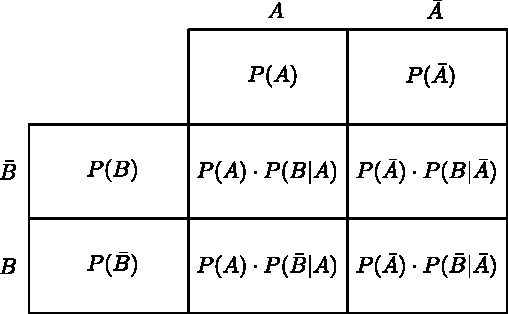
\includegraphics[width=1\textwidth]{bedingte-wahrscheinlichkeit.pdf}
	\end{subfigure}

	\rule[1mm]{0mm}{5mm}

	\begin{subfigure}[b]{0.75\textwidth}
		\centering
		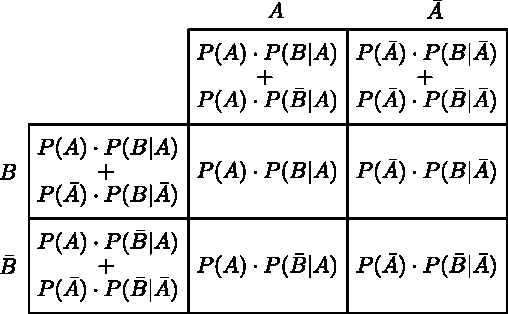
\includegraphics[width=1\textwidth]{bedingte-wahrscheinlichkeit-detail.pdf}
	\end{subfigure}
	\caption{Tabelle bedingter Wahrscheinlichkeiten.}
\end{figure}

\newpage
\begin{figure}[h!]
	\centering
	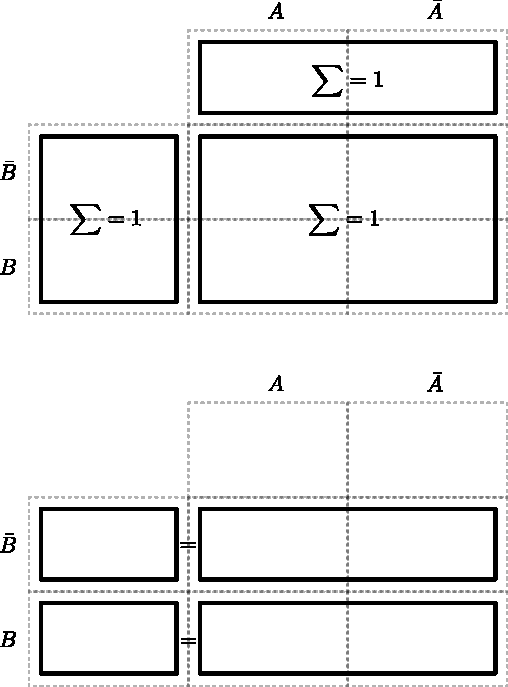
\includegraphics[width=0.65\textwidth]{bedingte-wahrscheinlichkeit-tipps.pdf}
	\caption{Hinweise zur Tabelle bedingter Wahrscheinlichkeiten.}
\end{figure}

